\section{Δίκτυα Ομότιμων Κόμβων} \label{section:2-4-p2p-networks}

Τα δίκτυα ομότιμων κόμβων ή Peer-to-Peer (P2P) networks αποτελούν μία κατανεμημένη αρχιτεκτονική δικτύων, οι συμμετέχοντες (κόμβοι) της οποίας μοιράζονται ένα τμήμα των πόρων τους, με στόχο την παροχή κάποιας υπηρεσίας (π.χ. τον διαμοιρασμό περιεχομένου). Εν αντιθέσει με συγκεντρωτικά δίκτυα τύπου client-server, οι κόμβοι (nodes) έχουν απευθείας πρόσβαση στους πόρους, χωρίς τη διαμεσολάβηση ενδιάμεσων οντοτήτων. Οι συμμετέχοντες ενός τέτοιου δικτύου είναι, δηλαδή, ταυτόχρονα, τόσο πάροχοι, όσο και αιτούντες των πόρων και της παρεχόμενης υπηρεσίας.\cite{2.4-p2p-networking}

\begin{figure}[H]
	\centering
	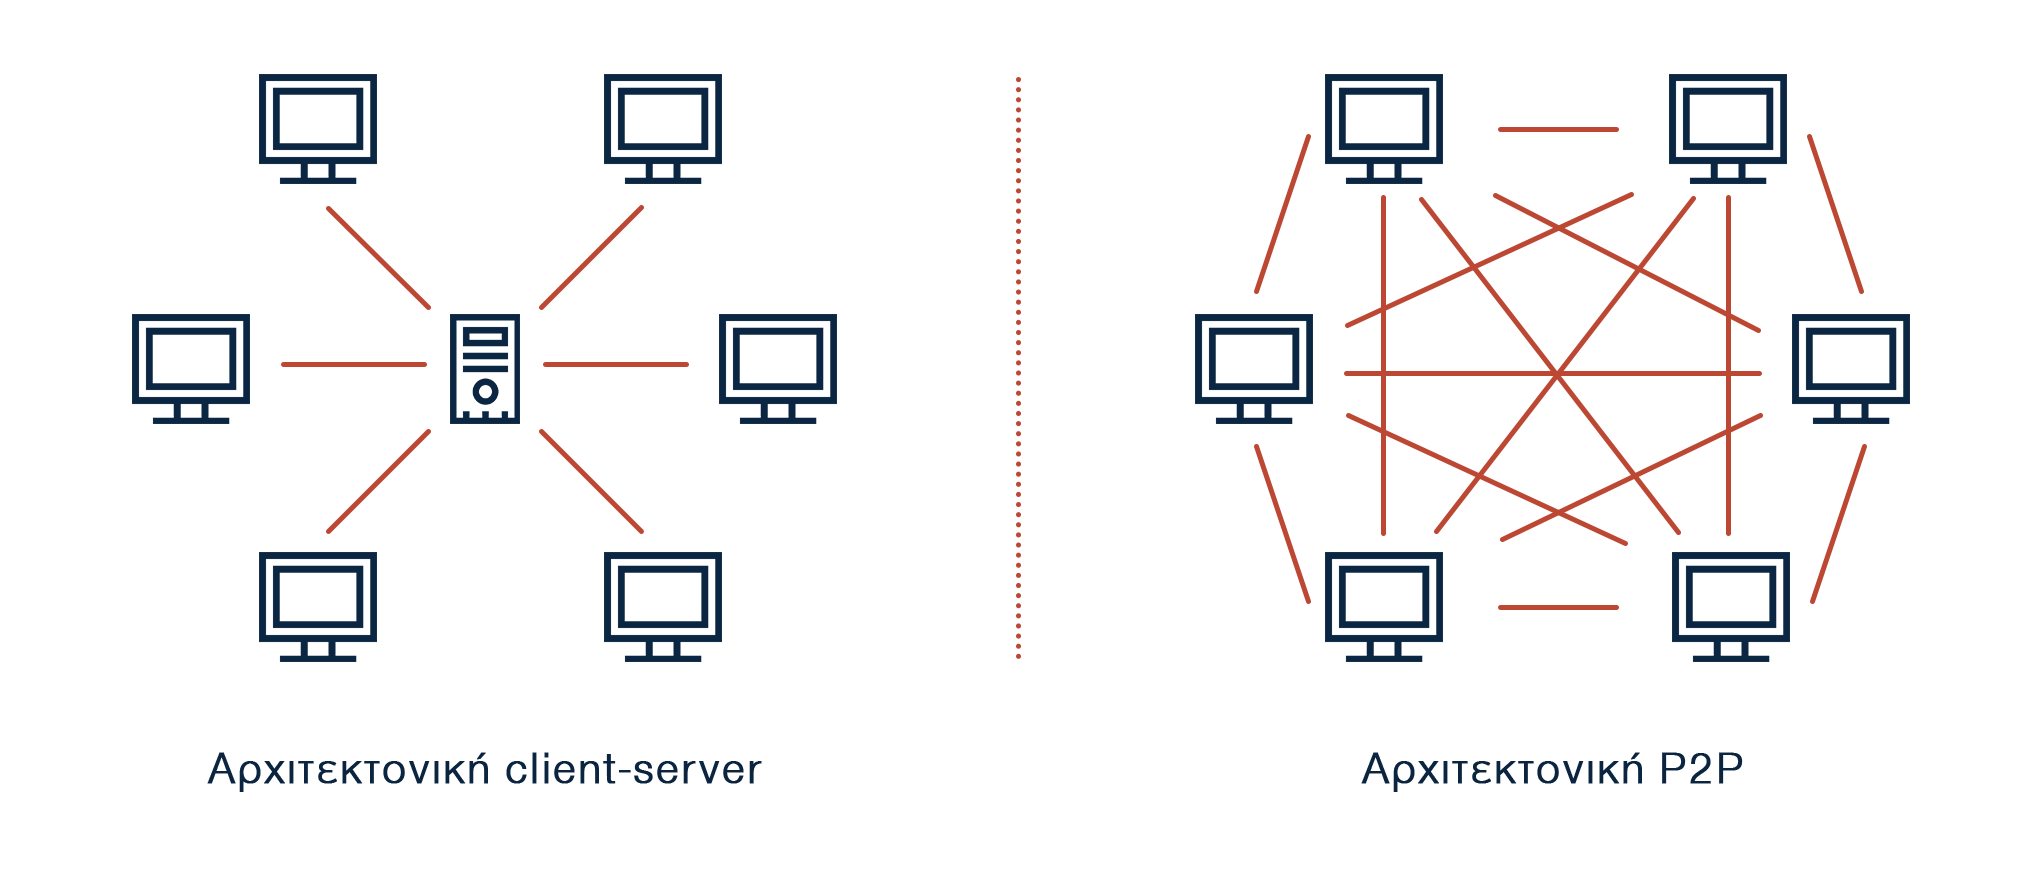
\includegraphics[width=.95\textwidth]{assets/figures/chapter-2/2.4.p2p-networks}
	\caption{Αρχιτεκτονικές δικτύων client-server και P2P}
\end{figure}

Τα P2P networks μπορούν να χωριστούν σε δύο κατηγορίες:

\begin{itemize}
	\item Στα "Καθαρά" (Pure) P2P networks, στα οποία ισχύει ότι η αφαίρεση ενός τυχαίου κόμβου από το δίκτυο δεν προκαλεί κάποιο πρόβλημα σε αυτό.
	\item Στα "Υβριδικά" (Hybrid) P2P networks, στα οποία συμμετέχουν επιπλέον και κεντρικές οντότητες, παρέχοντας απαραίτητα τμήματα των προσφερόμενων υπηρεσιών.
\end{itemize}

Από εδώ και στο εξής, εάν δεν αναφέρεται ρητά η κατηγορία κάποιου P2P network, θα εννοείται ότι ανήκει στην πρώτη.